\documentclass{beamer}

\usepackage[italian]{babel}
\usepackage[utf8]{inputenc}

\usepackage{graphicx} % Immagini fantastiche e...
\graphicspath{        % dove trovarle
  {./images/},
  %{../images/}        % Necessario se cartella chapters
}

%\usepackage{float}
%\usepackage{color}
%\usepackage{caption}
%\usepackage{subcaption}

%\usepackage{hyperref}
%\hypersetup{colorlinks=true, linkcolor=black, citecolor=black, plainpages=false, urlcolor=blue}
\usepackage{wallpaper}
%\usepackage{algpseudocode,algorithm,algorithmicx}
%\usepackage{amssymb}
%\usepackage{amsmath}
%\usepackage{lipsum} 


 
% ================================ %
%          Cose Personali          %
% ================================ %
\newcommand\E{\ensuremath{\mathbb{E}}}
\newcommand\T{\ensuremath{\mathbb{T}}}
\renewcommand\inf{\ensuremath{\infty}}



%%Information to be included in the title page:
\title{Approfondimento di Intelligenza Artificiale}
\author{Tristano Munini}
%\institute{Overleaf}
  %\LARGE{\underline{\textbf{ANNO ACCADEMICO 2019-2020}}}\\
%\logo{
\includegraphics{polloPallido}}



% ================================ %
%            Il Documento          %
% ================================ %
\begin{document}

{
  \usebackgroundtemplate{
    \centering
    
\includegraphics[width=\paperwidth]{polloPallido}
  }
  \frame{\titlepage}
}

\begin{frame}
\frametitle{Indice}
\begin{itemize}
  \item AutoEncoders (AE) e Variational AutoEncoders (VAE)
  \item Generative Adversarial Network (GAN)
  \item Reinforcement Learning (RL)
    \begin{itemize}
      \item QNN
      \item Policy Gradient
    \end{itemize}
  \item GAN + RL per generazione di testi
    \begin{itemize}
      \item SeqGAN
      \item LeakGAN
    \end{itemize}
\end{itemize}
\end{frame}

%\begin{frame}
%\frametitle{Introduzione}
%TODO
%\end{frame}

%\begin{frame}
%\frametitle{Riferimenti Esterni}
%cfr. MIT intro to deep learning
%\end{frame}

%%%%%%%%%%%%%%%%%%%%%%%%%%%%%%%%%%%%%%%%%%%%%%%%%%%%%%%%%%%%%%%%%%%%%%%%%%%%%%%%%%%%%%%%%%%%%%%%%%%
% AE and VAE
%%%%%%%%%%%%%%%%%%%%%%%%%%%%%%%%%%%%%%%%%%%%%%%%%%%%%%%%%%%%%%%%%%%%%%%%%%%%%%%%%%%%%%%%%%%%%%%%%%%
\begin{frame}
\frametitle{AutoEncoders}
$ x \in \textrm{real data space}$
\\
$ z \in \textrm{latent space}$
\\
$ \hat x \in \textrm{real data space}$


\begin{figure}[ht]
  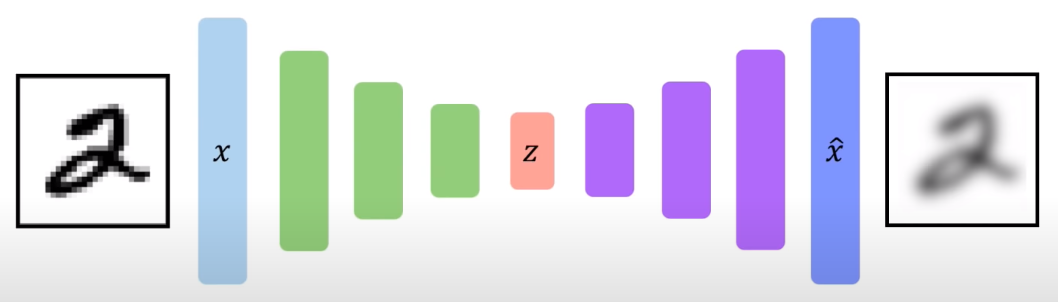
\includegraphics[width=\textwidth]{AE_01.png}
\end{figure}

The point of maximum compression, where $z$ is produced, is called bottleneck of the network

\end{frame}

\begin{frame}
\frametitle{Variational AutoEncoders}
$z$ is sampled from  the distribution with mean vector $\mu$ and standard deviation vector $\sigma$.
\\
We want an $\hat x$ that is similar to $x$ but that has some differences.
We want a variation of $x$.
\begin{figure}[ht]
  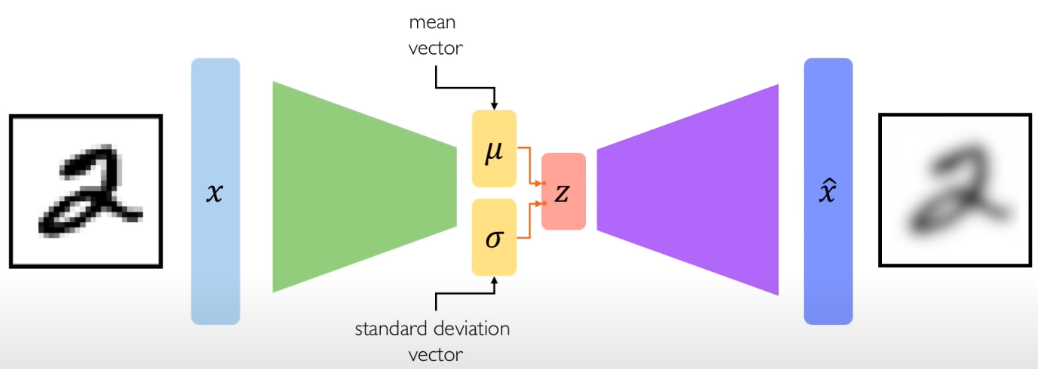
\includegraphics[width=\textwidth]{VAE.png}
\end{figure}
\end{frame}

\begin{frame}
\frametitle{Reparametrization Trick}
We can not use $z \sim \mathcal{N}(\mu, \sigma ^ 2)$
\\
So we use
\begin{align*}
  z = \mu + \sigma \odot \varepsilon
  \quad \textrm{where $\varepsilon  \sim \mathcal{N}(0,1)$}
\end{align*}
Where $\odot$ notes the element-wise multiplication
\\
Now $z$ is the sum of two fixed vectors, $\mu$ and $\sigma$, and a random constant $\varepsilon$ used as a weight

%\begin{figure}[ht]
%  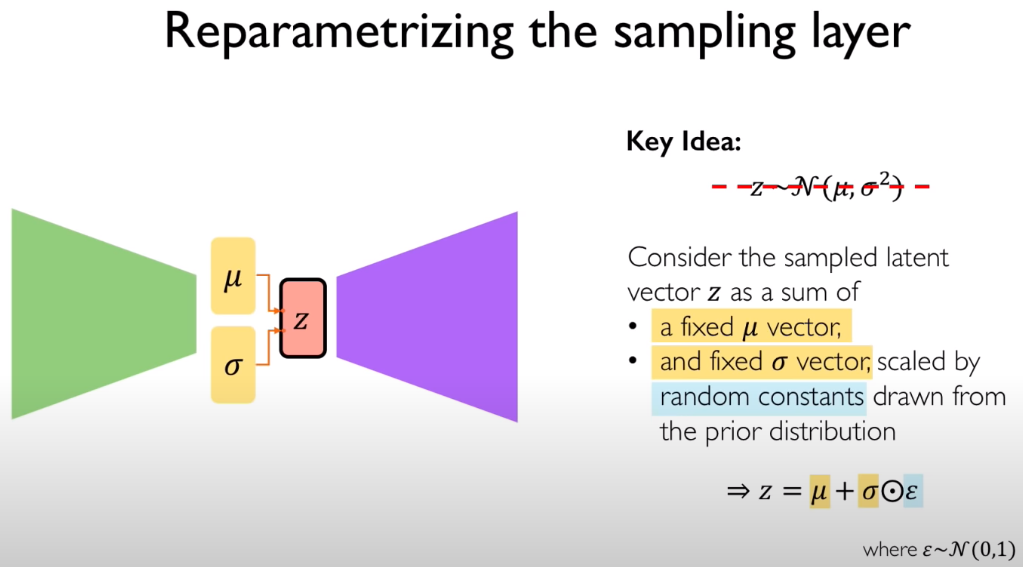
\includegraphics[width=\textwidth]{VAE_reparam_trick.png}
%\end{figure}
\end{frame}

\begin{frame}
\frametitle{Reparametrization Trick}
\begin{figure}[ht]
  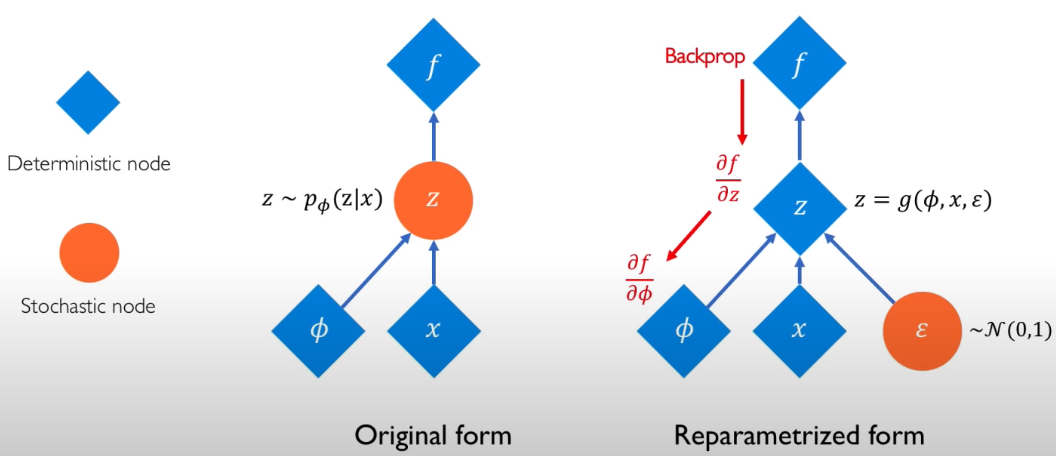
\includegraphics[width=\textwidth]{VAE_reparam_trick_backprop_01.png}
\end{figure}
\end{frame}

%%%%%%%%%%%%%%%%%%%%%%%%%%%%%%%%%%%%%%%%%%%%%%%%%%%%%%%%%%%%%%%%%%%%%%%%%%%%%%%%%%%%%%%%%%%%%%%%%%%
% GAN
%%%%%%%%%%%%%%%%%%%%%%%%%%%%%%%%%%%%%%%%%%%%%%%%%%%%%%%%%%%%%%%%%%%%%%%%%%%%%%%%%%%%%%%%%%%%%%%%%%%
\begin{frame}
\frametitle{Generative Adversarial Networks}
GANs are a way to make a generative model by having two neural networks compete with each other
\begin{figure}[ht]
  %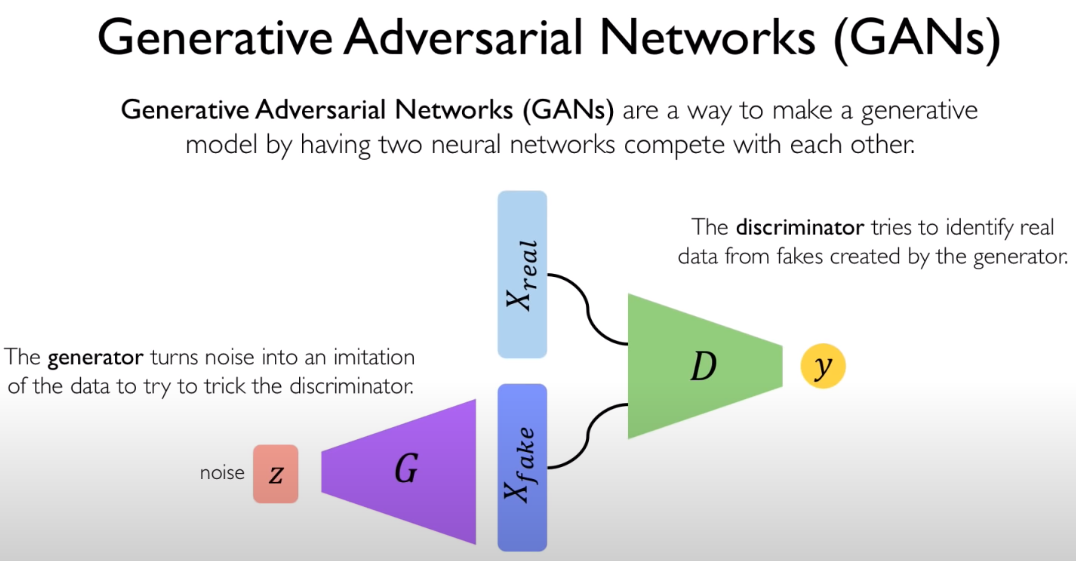
\includegraphics[width=\textwidth]{GAN.png}
  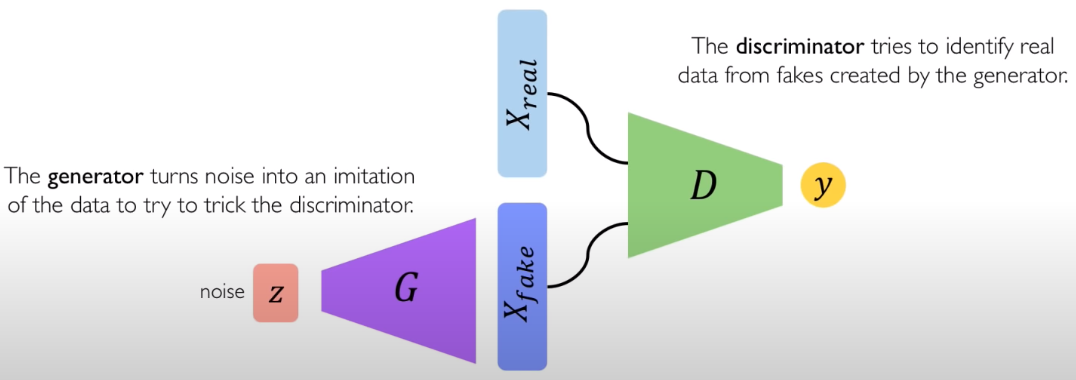
\includegraphics[width=\textwidth]{GAN_01.png}
\end{figure}
$z$ can be sampled form $\mathcal{N}(0,1)$ as in the VAEs
\end{frame}

\begin{frame}
\frametitle{GAN Training}
It is a min-max game
\begin{align*}
  min_G \, max_D \: V(D,G) &=
    \E_{x \sim P_{real(x)}} [ log D(x) ]
    \\                     &+
    \E_{z \sim P_z(x)} [ log ( 1 - D(G(z)) ]
\end{align*}
Where $P_{real(x)}$ is the probability distribution of the real data and $P_z(x) = \mathcal{N}(0,1)$ in our case

\end{frame}

\begin{frame}
\frametitle{GAN Problems}
\begin{itemize}
  \item Hard to converge to a good solution
  \item Vanishing gradient problem
  \item Model collapse
  \item Hard to find equilibrium
\end{itemize}
\end{frame}



%%%%%%%%%%%%%%%%%%%%%%%%%%%%%%%%%%%%%%%%%%%%%%%%%%%%%%%%%%%%%%%%%%%%%%%%%%%%%%%%%%%%%%%%%%%%%%%%%%%
% RL
%%%%%%%%%%%%%%%%%%%%%%%%%%%%%%%%%%%%%%%%%%%%%%%%%%%%%%%%%%%%%%%%%%%%%%%%%%%%%%%%%%%%%%%%%%%%%%%%%%%
\begin{frame}
\frametitle{Reinforcement Learning}
\begin{figure}[ht]
  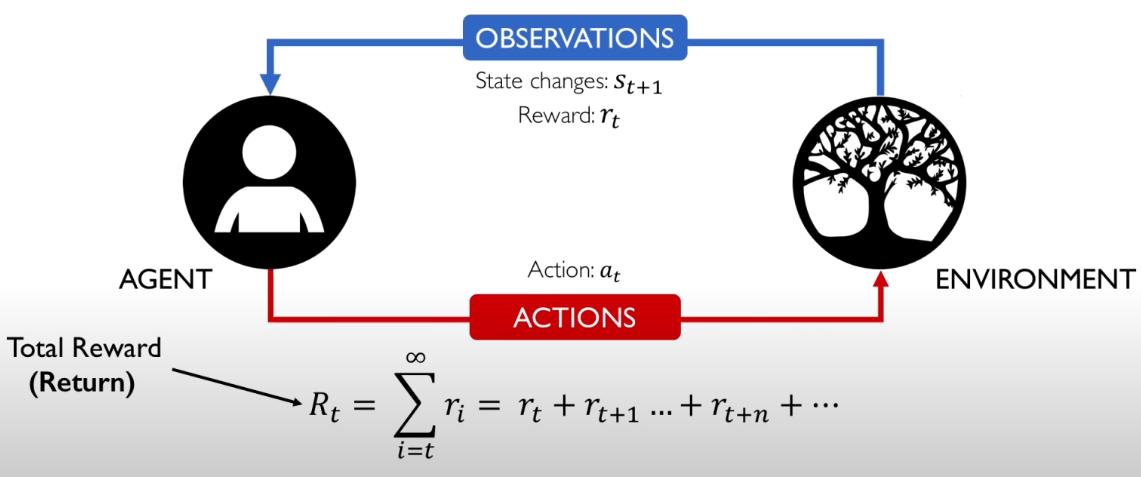
\includegraphics[width=\textwidth]{RL_key_concept.png}
  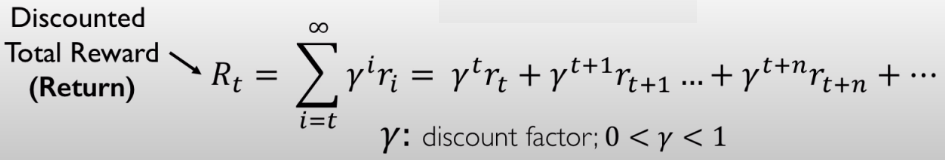
\includegraphics[width=\textwidth]{Discounted_Total_Reward.png}
\end{figure}
\end{frame}

\begin{frame}
\frametitle{template}
\begin{figure}[ht]
  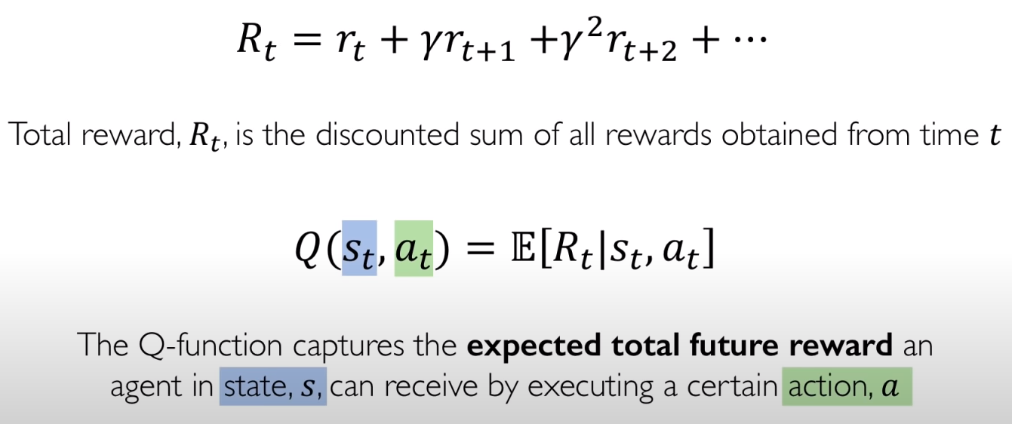
\includegraphics[width=\textwidth]{Q-Function.png}
  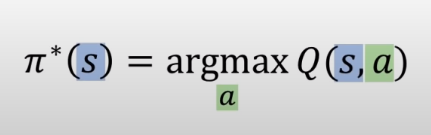
\includegraphics[width=.5\textwidth]{Policy_Fun.png}
\end{figure}
\end{frame}


%\begin{frame}
%\frametitle{template}
%\begin{figure}[ht]
%  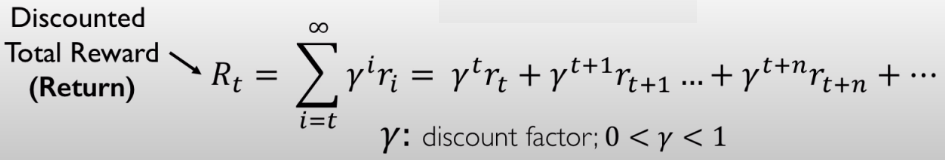
\includegraphics[width=\textwidth]{Discounted_Total_Reward.png}
%  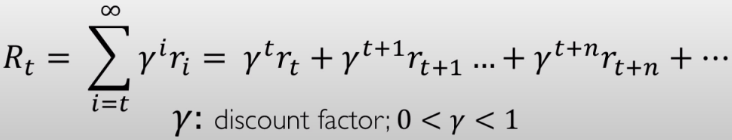
\includegraphics[width=\textwidth]{Discounted_Total_Reward_Formula.png}
%\end{figure}
%\end{frame}

\begin{frame}
\frametitle{template}
\begin{figure}[ht]
  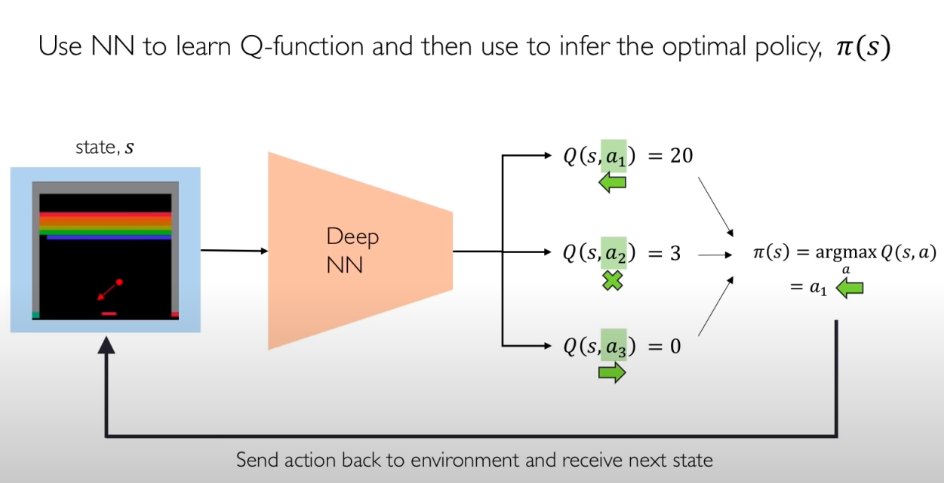
\includegraphics[width=\textwidth]{QNN.png}
\end{figure}
\end{frame}

\begin{frame}
\frametitle{template}
\begin{figure}[ht]
  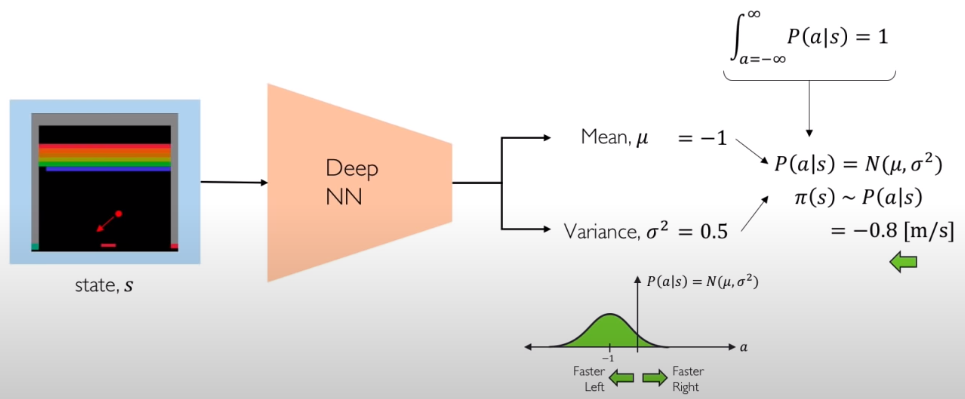
\includegraphics[width=\textwidth]{Pol_Grad.png}
\end{figure}
\end{frame}


\begin{frame}
\frametitle{template}
\begin{figure}[ht]
  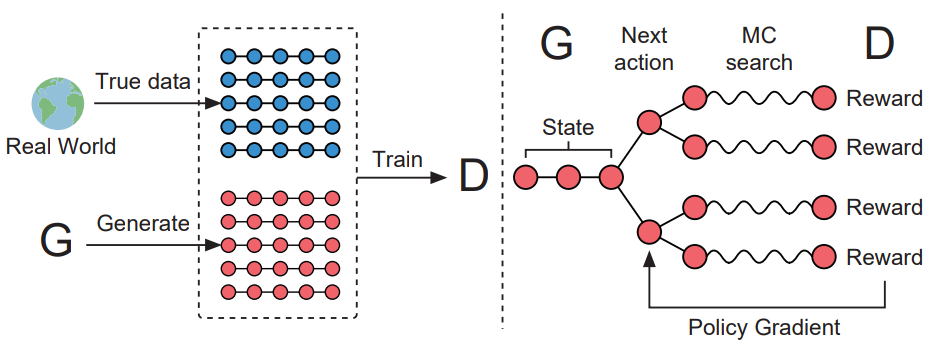
\includegraphics[width=\textwidth]{SeqGAN_Idea.png}
  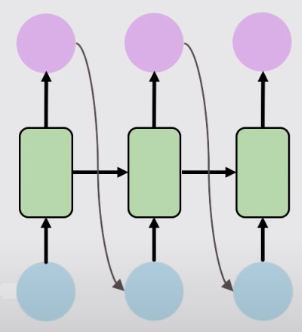
\includegraphics[width=.2\textwidth]{RNN.png}
\end{figure}
\end{frame}

%\begin{frame}
%\frametitle{template}
%\begin{figure}[ht]
%  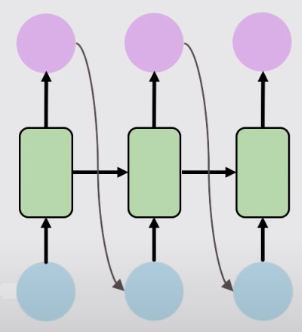
\includegraphics[width=\textwidth]{RNN.png}
%\end{figure}
%\end{frame}

\begin{frame}
\frametitle{template}
\begin{figure}[ht]
  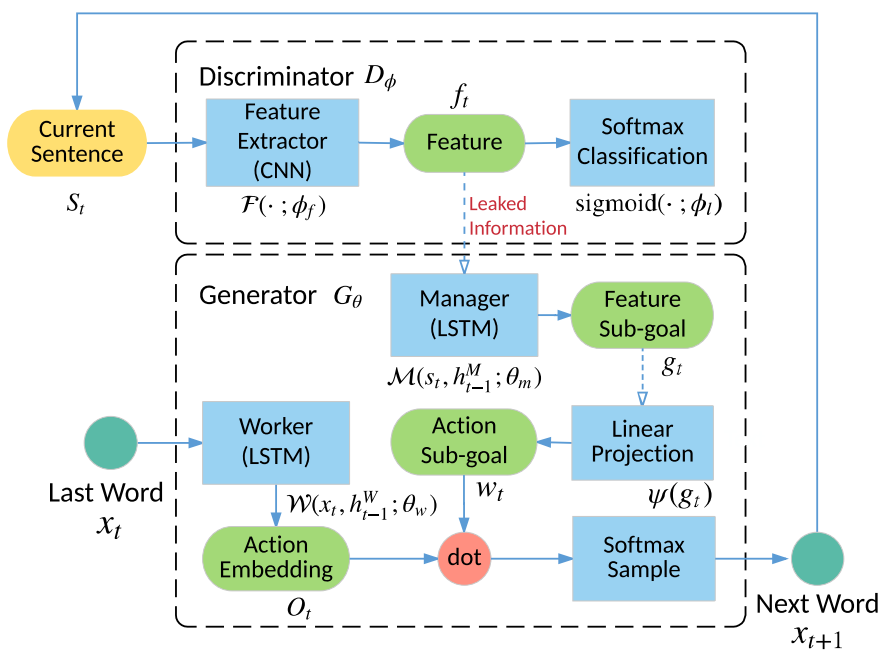
\includegraphics[width=\textwidth]{LeakGAN_Arch.png}
\end{figure}
\end{frame}

\begin{frame}
\frametitle{template}
\begin{figure}[ht]
  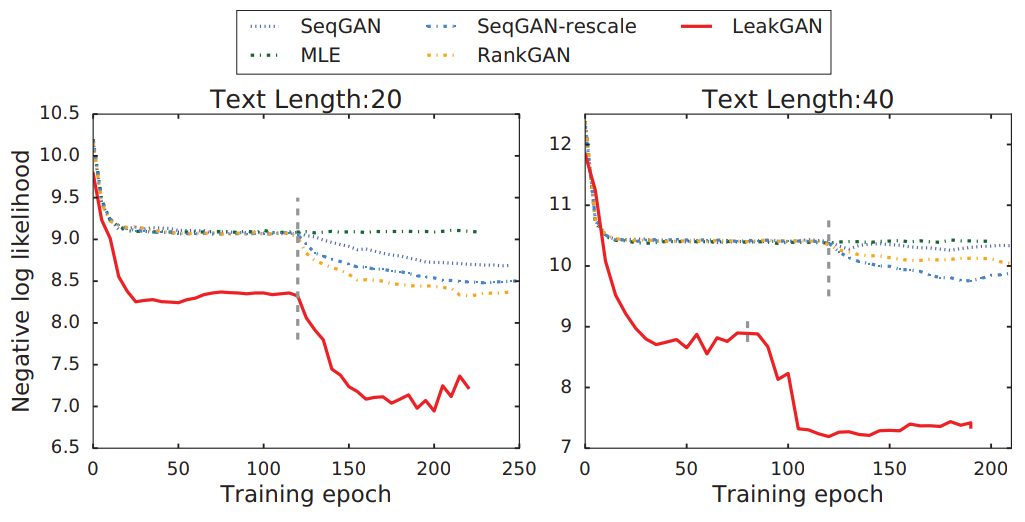
\includegraphics[width=\textwidth]{LeakGAN_vs_SeqGAN.png}
\end{figure}
\end{frame}

% AE.png
% 
% VAE.png
% VAE_reparam_trick_backprop.png
% VAE_reparam_trick.png
% 
% GAN.png
% 
% RL_key_concept.png
% Q-Function.png
% 
% Discounted_Total_Reward.png
% Discounted_Total_Reward_Formula.png
% QNN.png
% 
% Policy_Fun.png
% Pol_Grad.png
% 
% SeqGAN_Idea.png
% RNN.png
% 
% LeakGAN_Arch.png
% LeakGAN_vs_SeqGAN.png






\end{document}
